\chapter{Collective Communication}
\section{What are Collective Communications ?}
In the previous chapter we have briefly described the basic {\tt SCU} 
calls for nearest neighbour point to point communication. This 
kind of communication is fine if we want to program communications
between processors that are reminiscent of the HPC {\tt CSHIFT} 
function for example, or if we wish to build systolic array like 
systems.

Occasionally however we may want to perform certain global communications
such as a sum of data items held across all the processors. An immediate
example of such a situation is the case of taking the scalar product of two vectors. Imagine that the vector
components are distributed amongst the nodes of the parallel computer. Each 
processor could work out the sum of the squares of its local vector components
but to accumulate the dot product, these local results would have to be
globally summed. 

\section{Who Communicates?}
The distinguishing feature of global communications also known
sometimes as collective communications is that all the processors make
the call to the communication routines, whereas in the case of a point
to point communication, usually only the sending and the receiving
node call a communication routine.

In the case of MPI and other message passing standards usually one has
a way of selecting subgroups of processor nodes from a given available
set. In MPI for example the so called 'communicator' {\tt
MPI\_COMM\_WORLD} refers to all available processors and subgroups of
these can be identified by defining new communicators (using such
routines as {\tt MPI\_Comm\_split}.)

In the case of the QCDSP, selecting processor partitions is non
trivial. Machines are often 'manually hardware partitioned' ( a
technical process involving graduate student plugging wires on the
backplanes of crates ).  Alternatively, in a given hardware partition,
one may select a certain set of processors using the QOS command {\tt
qset\_nodes }.  Once a given set of nodes is selected by either method
however, it is non--trivial to sub--select again from within a running
program.  Consequentially, our description of collective
communications will refer to situations when all available processor
nodes take part in the communication. These kinds of collective
communications are referred to as global communications. From here on
we shall use the two phrases interchangeably.

\section{Global Communication in General}
We now describe some common types of collective communication.
Since a lot of these are in the MPI message passing interface
specification I shall refer frequently to MPI equivalents. If
you know MPI this should make things easy for you. It should
also clear up ambiguities (I hope) in other situations.

\subsection{Barrier} 
A {\em barrier} routine is used to synchronise a set of processors.
All the nodes call the barrier routine. The routine does not exit
until all the processes participating in the communication have
entered it. In MPI one would require a call to the function {\tt
MPI\_Barrier}. In the case of the QCDSP the functionality is provided
through the system call {\tt sync()}, which is defined in the system
header file {\tt sysfunc.h}.

\subsection{Broadcast}
There are two general kinds of broadcast routines. They are 
\begin{description}
\item{\bf One To All Broadcast: \ }
This is procedure where a given processor node (usually referred to as
the root processor) contains some information. This information 
is sent to all other processors during a one to all broadcast routine.
\item{\bf All to All Broadcast: \ }
This is a procedure where at the outset each processor has an item
of data, and during the broadcast procedure each processor makes available
its data to all other processors. At the end of the broadcast, all
the processors are in possession of the data elements from all the other
processors.
\end{description}

The idea of the two kinds of broadcasts are illustrated in figures
\ref{f:oneToAllBroadcast} and \ref{f:allToAllBroadcast} respectively.
\begin{figure}[h]
\begin{center}
\leavevmode
\hbox{%
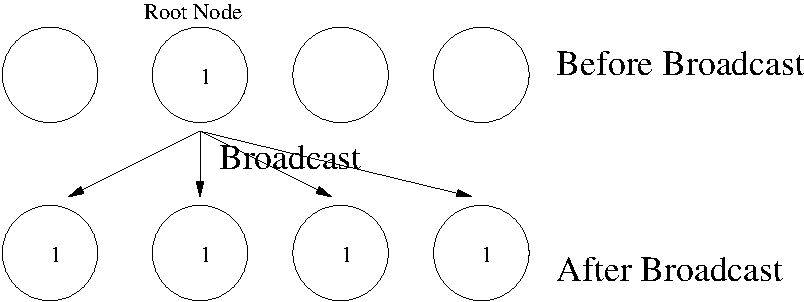
\includegraphics{one_to_all_bcast}
}
\end{center}
\caption{One to all broadcast. The circles represent
processor nodes. Before the broadcast, the root node holds the data
item to be distributed, in this case the number 1. After the
broadcast, the data item is found on all processors}
\label{f:oneToAllBroadcast}
\end{figure}

\begin{figure}[h]
\begin{center}
\leavevmode
\hbox{%
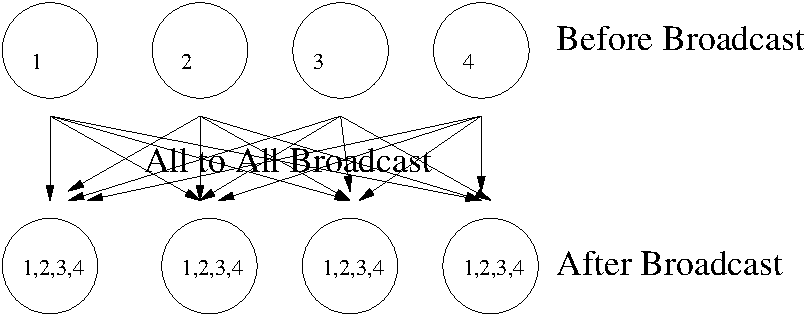
\includegraphics{all_to_all_bcast}
}
\end{center}
\caption{All to all broadcast: The circles represent processor nodes.
Before the broadcast all items hold their own data (the numbers inside 
them). After the broadcast, each processor has a copy of everybody 
else's data.}
\label{f:allToAllBroadcast}
\end{figure}

Important uses of broadcast operations can include the distribution
of parameters from a source processor as well as situations where 
one processor has to be a 'master' and has to make global decisions.
These decisions then probably need to be broadcast out to the other processors.

\subsection{Gather and Scatter}
The {\em gather} operation is one in which all processors send their
data to a nominated root processor. Its opposite is the so called 
{\em scatter operation} where the nominated root processor distributes
a vector of data, to the whole processor grid. The operations are illustrated
in figure \ref{f:gatherscatter}.
\begin{figure}
\begin{center}
\leavevmode
\hbox{%
\includegraphics{gatherscatter}
}
\end{center}
\caption{Above: Scatter operation. One processor 'scatters' its data
amongst the complete set. Below: Gather operation: The data from all
processors is 'gathered' onto a root processor.}
\label{f:gatherscatter}
\end{figure}
Sometimes the terms {\em gather} and {\em scatter} are generalised, to
mean that one processor distributes its data to some subset of other
processors (for example its nearest neighbours in the processor
grid). In this sense the corresponding gather would be the collection
of data from the same subset of processors.

In fact the broadcast operation can be implemented as a scattering
operation, where all processors receive the same data item. Likewise
the neighbour discovery exercise at the end of the last exercise (have
you attempted it?)  is an example where we combine a generalised
gather and a generalised scatter.  The generalised gather is that each
node (of a given parity) receives the processor ID of its nearest
neighbours, whereas the generalised scatter is the part where every
node (of the opposite parity) sends its ID to its nearest
neighbours. The MILC collaboration, in their code\footnote{Freely available at {\tt  http://cliodhna.cop.uop.edu/\~hetrick/milc/}. You could do us a great
service if you ported it to the QCDSP...} has refined the
generalisation of gathering and scattering to such a level where a
user can actually define his or her own gather and scatter mapping.

Scatter and Gather operations are useful for example to distribute data
that has just been read from disk by a master processor (assuming of course
that the master processor can hold all the data in memory) or to pass out
processor specific decisions. It can also be used, as mentioned before
to implement the broadcast operation. Generalised scatters can be useful
for exchanging data boundaries between processors for example.

\subsection{Global Reduction}
Global reduction operations generally take data from each node and
produce one single (reduced) result. Examples of global reduction are
global sums, global products, global XOR operations, finding global
minima and maxima. In fact any associative operation can be used as a
reducing operation. It perhaps for this reason that MPI has only two
functions {\tt MPI\_Reduce} and {\tt MPI\_Allreduce} to carry out all
their reduction operations\footnote{The actual operation and type of
data are specified using tags such as {\tt MPI\_INT} and {\tt MPI\_SUM}
for example}, instead of having separate global sum, global XOR and
other global routines.
 
Once again there are two kinds of global reduction operations.
\begin{description}
\item{\bf All to One Reduction: \ } -- these are reduction operations
where the final answer is left with one nominated (root) processor. 
These correspond to {\tt MPI\_Reduce}.
\item{\bf All to All Reduction: \ } -- these are reduction operations
where the final answer is given to every processor. These correspond 
to {\tt MPI\_Allreduce}. 
\end{description}

It should be clear for example that one can implement all to all 
reduction operations as an all to one reduction operation followed 
by a broadcast.

An important use of global sums for example is in the computation
of scalar products. A use of a global maximum operation for example
would be to find the infinity norm of a distributed vector. Global
XOR operations may be needed for checksumming a distributed dataset.
A quick and dirty floating point broadcast routine could be written
using a global sum where the root node contributes to the sum the 
amount it wishes to broadcast and all the other processors contribute
0. 

A {\bf warning} about global sums and other global operations which
are susceptible to cancellation errors and or bit overflow problems:
The QCDSP system can contain anything from between 64 nodes to
O($10^5$) nodes. Even if a single node has only component to contribute
to a particular reduction, it is possible that when for example 16K 
processors are involved in an operation there is a serious chance
of overflow or that cancellation errors have a serious effect.
There are two ways to address this problem:
\begin{itemize}
\item
The implementors should implement their reduction operations in 
such a way as to minimise the problems of rounding error accumulation/
overflow/underflow. They could for example carry out sums in a logarithmic
manner etc.
\item
The implementors could throw extra bits of precision at the problem,
and provide status registers indicating overflow underflow. 
\end{itemize}

\section{Global Communication on the QCDSP}
The QCDSP was designed to run simulations of lattice QCD. The predominant
communication pattern for this application is nearest neighbour, with
the occasional need for global operations. In fact lattice QCD does
not really require more in terms of communications than
broadcasts, nearest neighbour gather and scatter operations, global
sums, global minima and maxima. 

Consequentially, the design of the hardware and the software reflect
these needs. The hardware design is such as to favour efficient
nearest neighbour communications. Although the hardware does have
support for performing global reduction operations, accessing them is
not entirely straightforward. Also, since these global reduction
operations were found not to be a major performance bottleneck, little
effort has been made to optimise them. Even worse, the global
communication routines that are optimised are part of the
Columbia/Brookhaven Physics system and are not available for general
use.

Distributed data is loaded to the processors by the QOS before applications
start running. (More details in the Chapter on I/O) This sidesteps the
need for routines that gather and scatter data to and from some
root processor for the purposes of file I/O. Furthermore these are not
entirely straightforward for a general user to code up as there is no
hardware support for routing a message from any given processor to the
root processor directly. An implementer would have to pass the message 
through intermediate processors, which are neither senders nor receivers
of this information possibly having to stop computation on the intermediate
processors for this purpose.

All that remains for a user to implement then are global reduction
routines and broadcasts. We now look at some algorithms for
performing these global communications. We then present a simple
library that performs global sums, minima and maxima for numbers of
type {\tt float}. Users are welcome to use this library in their own
programs, or can use the library merely as an example to aid in
writing their own routines.

\section{Global Reduction Algorithms for Ring Architectures}
We now discuss some global reduction algorithms for 1D ring architectures.
A 1D ring is simply a set of processors connected in series with 
wrap around edges at the ends of the line. A picture of a ring can
be seen in figure \ref{f:1Dring}.
\begin{figure}
\begin{center}
\leavevmode
\hbox{%

\includegraphics{1Dring}
}
\end{center}
\caption{A 1D ring. The circles represent processors and the lines
represent connections.}
\label{f:1Dring}
\end{figure}

Although the QCDSP has a network connectivity that is a four dimensional 
torus it can also be viewed as a collection of rings. We illustrate
the idea for a two dimensional torus in figure \ref{f:TorusRing}.
Here we can look at a two dimensional torus as a collection of rings in
either the {\em x} or {\em y} directions
\begin{figure}
\begin{center}
\leavevmode
\hbox{%
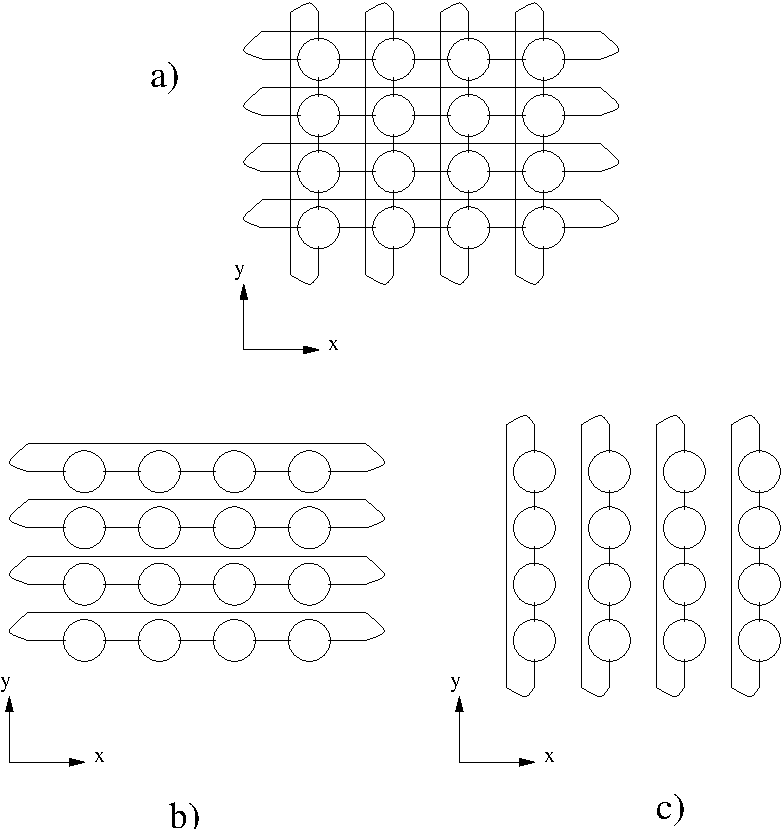
\includegraphics{torusRing}
}
\end{center}
\caption{(a)A 2D torus as a set of 1D rings in the (b) {\em x} direction and (c) the {\em} direction}  
\label{f:TorusRing}
\end{figure}

One general way of programming global reduction algorithms on a 4D mesh
is to perform the operation first on all rings in the {\em x} direction,
then on all the rings in the 'y' direction and so on in the remaining two
directions. 

\subsection{Ring all to all reduction algorithm}
Consider the following reduction algorithm:

Each processor in the ring sets up a buffer to store the result of the
reduction. The result buffer is initialised with the processors own data.

Each ring then transmits its data in one direction along the ring
and receives data from the opposite direction. (We shall refer to these 
as the positive and negative directions respectively). The data that
has been received is combined with the data in the result buffer, to 
generate a new intermediate result..

The process of transmitting the local data in the positive direction
and receiving data from the negative direction and combining it with the
result is repeated until each data item has visited each processor once.
For a ring containing $n$ processors exactly $n-1$ steps are needed.
When all the steps are complete, the result buffer should contain the
final answer.

The process is illustrated for addition in a 4 processor ring in figure
\ref{f:ring_addition}.
\begin{figure}
\begin{center}
\leavevmode
\hbox{%
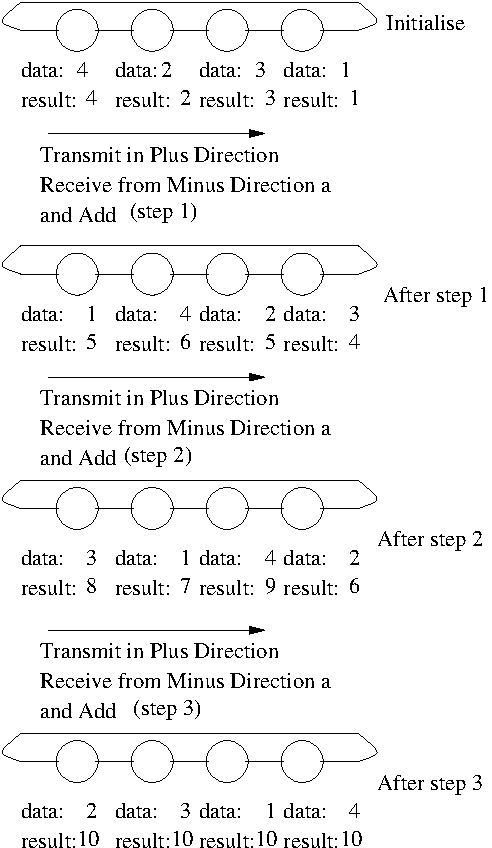
\includegraphics{1Dring_addition}}
\end{center}
\caption{1D Ring Addition Algorithm: At each step data is passed in 
the positive direction (right) and received from the negative direction (left).
The data is then added to the results buffer. After 4-1 = 3 steps
all the processors have the global sum}
\label{f:ring_addition}
\end{figure}

Note that in this particular algorithm, each processor performs the
sum in a different order from its neighbour. This is one of the
reasons why reduction operations need to be associative. Also since
floating point arithmetic is not really associative due to roundoff
errors, it is possible that rounding errors will affect different
processors differently and for a floating point global sum using the
above algorithm, it is possible that the answers on individual
processors are not bit-identical.

This can be a problem for example if one is trying to decide whether one 
meets the stopping criteria for some iterative process based on the result
of a global sum (such as in the case of an iterative solver, where the 
stopping criteria depends on a scalar product). Clearly it is possible
that some processors meet this criteria and some, due to rounding errors
do not. 

The problem can be solved by nominating one processor as the master of
the others. The decision as to whether to stop the solver will then
depend on the result held by the master node. One can either broadcast
the master's result and let each processor make its decision based on
that, or alternatively the master can make the decision and broadcast
it instead in the form of a token, a flag or in some other encoding.
Alternatively one can formulate the global sum so that the results are
guaranteed to be bit identical across all the processors, say by using
a different algorithm where the sum is first reduced to some single root 
processor in all the rings which then transmit the sum back along their
respective rings before going on to the next dimension.

\subsection{Mesh Global reduction algorithm}
As mentioned before, the generalisation of the ring algorithm to the 
mesh is simply to perform the global operation along each ring in
parallel for a given direction, and to repeat this process for 
all directions. 

Figure \ref{f:2DMeshsum} shows the idea for a two dimensional mesh.
\begin{figure}
\begin{center}
\leavevmode
\hbox{%
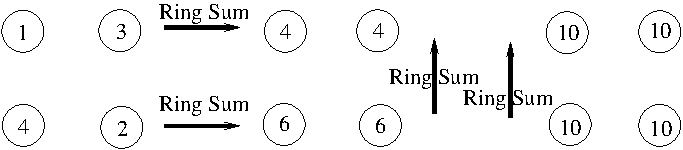
\includegraphics{mesh_sum}
}
\end{center}
\caption{2D Mesh Global sum. First the sum is performed along both 
rings in the horizontal direction. Second it is performed along 
both rings in the vertical direction.}
\label{f:2DMeshsum}
\end{figure}

\subsection{Coding the Routines For the QCDSP}
We show below the QCDSP C++ code for finding the global maximum
using similar the algorithms described above.
\begin{verbatim}
// ------------------------------------------------------
// Include Files
// ------------------------------------------------------
#include <glb.h>
#include <sysfunc.h>

// ------------------------------------------------------
// Macros for picking local min/max
// ------------------------------------------------------
#define max(A, B) ((A) > (B) ? (A) : (B))

// -------------
// Buffer space 
// -------------
static float transmit_buf;
static float receive_buf;
static float max_buf;

// ------------------------------------------------------
// Function glb_max
//
// Argument: A pointer to the local number that is to
// be considered for being the Global Maximum. At the end
// of the function, the pointer points to the global maximum
// ------------------------------------------------------
void glb_max(float * float_p)
{
  // ---------------------------------------------
  // Size of the Processor Grid in each dimension
  // ---------------------------------------------
  int NP[4] = {SizeT(), SizeX(), SizeY(), SizeZ()};

  // ---------------------------------------------
  // Array to hold SCU send and receive directions
  // We will later index into this.
  // ---------------------------------------------
  const SCUDir dir[] = { SCU_TP, SCU_TM, SCU_XP, SCU_XM,
                         SCU_YP, SCU_YM, SCU_ZP, SCU_ZM };
  // ---------------------------------------------
  // Place the local number in the comparison buffer
  // ----------------------------------------------
  max_buf = *float_p;

  // ----------------------------------------------
  // Loop over the processor grid dimensions
  // ----------------------------------------------
  int dim;
  for(dim = 0; dim < 4; dim++) {

      // -----------------------------------------
      // Send our local minimum in the +ve direction
      // (NP[ 2 * dim ]) direction and receive from the
      // -ve (NP[ 2 * dim ]) direction with wraparound
      // at the pe grid boundary. Do this NP - 1 times
      // so that everyone can compare everybody's data
      // in this dimension
      // -----------------------------------------
      transmit_buf = max_buf;

      int tmp;
      for (tmp = 1; tmp < NP[ dim ]; tmp++) {
        // -----------------------------------------
        // Set up the communications handles:
        // -----------------------------------------

        SCUDirArg send(&transmit_buf, dir[ 2*dim ],
                       SCU_SEND, sizeof(float));
        SCUDirArg rcv(&receive_buf, dir[ 2*dim+1 ],
                      SCU_REC, sizeof(float));


        // -----------------------------------------
        // Perform the transfers
        // -----------------------------------------
        SCUTrans(&send);
        SCUTrans(&rcv);

        SCUTransComplete();

        // -----------------------------------------
        // Keep the maximum of what you had and what
        // you just received
        // -----------------------------------------
        max_buf = max(max_buf, receive_buf) ;

        // -----------------------------------------
        // Pass on the received data
        // -----------------------------------------
        transmit_buf = receive_buf;
      }
  }

  // --------------------------
  // Store the global max
  // --------------------------
  *float_p = max_buf;
}
\end{verbatim}
The global minimum and sum routines would follow a similar pattern.

\section{A simple collective communications library}
In a manner similar to the {\em hello\_world} program a simple
global communications library is available on the QCDSP (once 
Bob puts it in place). It can be found in {\tt /qcdsp/sfw/qos.5.3.3/example/glb}.This directory has subdirectories {\tt include}, {\tt lib}, {\tt src} and {\tt test}. There is also a makefile in this directory of which more later.

The {\tt include} directory contains the file {\tt glb.h} which defines
the global communication subroutines. This has to be included in any 
user programs using the {\tt \#include} directive. The {\tt src} 
subdirectory contains the source files for the library plus a makefile
to build the libraries. The {\tt lib} directory is where the compiled
library gets placed after it is built in the {\tt src} subdirectory. 
This is the library that has to be linked with the user code and
is called {\tt glblib.olb} on the QCDSP. Finally, the {\tt test} 
directory contains a simple program that uses the library.

To build the library and the tests, go to the toplevel directory 
and type {\tt make all}. Once this process is finished, you should
find {\tt glblib.olb} in the {\tt lib} subdirectory and an
executable called {\tt glb\_test.out} in the {\tt test} subdirectory.

\subsection{The Library Routines}
The library provides the following routines.
\begin{description}
\item{ {\tt void glb\_sum(float * float\_p)} : \ } This routine
performs a global sum over all the processors. On entry, {\tt float\_p} 
should point to each node's own contribution to the sum. On exit
{\tt float\_p} will point to the result of the global sum. The algorithm
for the sum is as detailed in the last section. The sum is actually 
performed in 64 bits of precision through a user defined type. This
aspect of the operation is completely hidden from the user. At the 
end of the operation the result is rounded back to a 32bit result. 
\item{ {\tt void glb\_max(float * float\_p)} : \ } This routine 
finds the global maximum across all the processors. On entry {\tt float\_p}
points to the each processor's own data. On exit {\tt float\_p} points
to the maximum of these elements. This subroutine was listed explicitly in
the last section.
\item{ {\tt void glb\_min(float * float\_p)} : \ } This routine
finds the global minimum across all the processors. On entry {\tt float\_p}
points to each processor's own data. On exit {\tt float\_p} points
to the minimum of these elements.
\item{ {\tt void glb\_bcast(float * float\_p, int root\_id)} : \ } This 
routine broadcasts the number pointed to by {\tt float\_p} on the node
with unique ID {\tt root\_id} (as determined from {\tt UniqueID()}) to
all the processors.  The broadcast is implemented as a global sum with
node {\tt root\_id} contributing the number to be broadcast at the end
of {\tt float\_p} and all the other nodes contributing 0 to the sum.
\end{description}

We recommend that the reader takes a look at the source code to be
found in the {\tt src} subdirectory to look at the code for the above 
library routines. However most of them are similar to the global
maximum routine listed earlier.

\subsection{Using the Library}
We list below the test program from the {\tt test} subdirectory which 
shows all of the library routines in use. The program first sums the 
unique IDs of all the nodes, then finds the maximum and minimum of these.
Finally it broadcasts the ID's of each processor in turn and sums 
them accross the processor grid. The code is shown below:
{\small
\begin{verbatim}
#include <stdio.h>
#include <stdlib.h>
#include <sysfunc.h>
#include <glb.h>

int main(int argc, char *argv[])
{
  float sum_serial = 0;
  int i;

  // -----------------------------
  // Serial sum of processor ID's
  // -----------------------------
  for(i = 0; i < NumNodes(); i++) {
    sum_serial += (float) i;
  }

  // ----------------------------
  // Put Unique ID into buffer
  // ----------------------------
  static float my_buf = (float)UniqueID();

  // ----------------------------
  // Sum Unique IDs
  // ----------------------------
  glb_sum(&my_buf);

  // ----------------------------
  // Output results
  // ----------------------------
  printf("Serial Sum of IDs = %g  Global Sum = %g\n", sum_serial, my_buf);


  // ----------------------------
  // Find Minimum ID
  // ----------------------------
  my_buf = (float)UniqueID();
  glb_min(&my_buf);

  printf("Minimum Unique ID should be 0. It is %g\n", my_buf);

  // ----------------------------
  // Find Maximum ID
  // ----------------------------
  my_buf = (float)UniqueID();

  glb_max(&my_buf);

  printf("Maximum Unique ID should be %g. It is %g\n", 
         (float)(NumNodes()-1), my_buf);

  // ----------------------------
  // Do some broadcasting
  // ----------------------------
  for ( i = 0; i < NumNodes(); i++ ) {

    // -------------------------------
    // Process I will broadcast its ID
    // to everyone
    // -------------------------------
    if( UniqueID() == i ) {
      my_buf = (float)i;
    }
    else { 
      my_buf =(float) 200;
    }

    // -------------------------------
    // Broadcast with proc i as root: 
    // Should end up with i on each node
    // -------------------------------
    glb_bcast(&my_buf,i);
    
    // -------------------------------
    // Do a global sum on the result 
    // (should be NumElems()*i)
    // -------------------------------
    glb_sum(&my_buf);

    printf("Global sum of buffers should be %g. It is %g\n", 
          (float)(NumNodes()*i), my_buf);

  }
  return(EXIT_SUCCESS);

}
\end{verbatim}
}
When printing the result of each operation the program also prints
out what it expects the real result to be.

Why not compile up the library as indicated before and try out the test
program. On {\tt q\_1}, which is a 64 node development board I got
the following output.
\begin{verbatim}
Serial Sum of IDs = 2016  Global Sum = 2016
Minimum Unique ID should be 0. It is 0
Maximum Unique ID should be 63. It is 63
Global sum of buffers should be 0. It is 0
Global sum of buffers should be 64. It is 64
Global sum of buffers should be 128. It is 128
.
.
.
\end{verbatim}

\subsection{Using the Library in your own programs}
To use the library in your own programs you must do two things.
\begin{itemize}
\item
Firstly, you must include the header file {\tt glb.h} in every
source file that uses the routines.
\item
Secondly, you must link to the library {\tt glblib.olb}. This
may involve having to edit the Makefile. If you dislike this
idea (its not that bad really) simply copy the files ending in
{\bf .C} from the {\tt src} subdirectory into the directory 
you are working in. The default makefiles should compile
them up for you.
\end{itemize}

We shall say discuss compilation and linking in more detail in 
a later chapter. For now suffice it to say that both are done
using the {\tt tcpp} command. 

To include the {\tt glb.h} header file, it is perhaps easiest 
if you leave it in some sensible (Perhaps Bob will leave it
in a sensible place where it can stay forever). You can then do 
one of two things.
\begin{itemize}
\item
You can include it with the directive {\tt \#include "sensible\_path/glb.h"}
where for {\tt sensible\_path}, you should substitute the path
of the sensible place where the header file lives.
\item
You can include it with the directive {\tt \#include <glb.h>}. In this
case you have to make sure that the compiler will look in the sensible
place where the {\tt glb.h} file is by default. You can specify
a list of directories for the compiler to search with the {\tt -i}
compiler flag.
\item
If you feel really unhappy about either of the above options you can
always copy the {\tt glb.h} file into the directory that you are working
in and just include it as {\tt \#include "glb.h"}. This way you need
neither edit the makefile nor mess with compiler flags. Its the 
chicken way out tho' and it may leave you open to having
different versions of the header file in different projects. A real
nightmare...
\end{itemize}
I prefer the latter method personally, as then I only have to 
type the name of the directory in which the file lives once, in
the makefile.

However I do repeat: {\bf If you fear and loath makefiles, do not
panic for we shall clarify them in a later chapter. Until then, just
copy the files from the {\tt src} subdirectory and {\tt glb.h} to the
directory where you are coding and use the default makefiles.}

\section{Summary of Chapter}
In this chapter, we have discussed collective communications.
After outlining some of the most common global communication techniques,
the barrier, the broadcast, gather, scatter and reduction operations
we discussed which of these may be implemented on the QCDSP. 
We then outlined some simple algorithms for performing global reduction
operations on a mesh parallel architecture. Finally, we discussed a
simple library for the QCDSP which defines global sums, maxima and minima
for floating point numbers.

\section{Exercise}
Can you think of more efficient ways of doing global sums on the 
QCDSP ? You should be able to get some ideas from the QCDSP WWW page:
{\tt http://www.phys.columbia.edu/\~cqft/qcdsp.htm} where they describe
the hardware support for global sums. You can also get some ideas
from the book ``Introduction to Parallel Computing'' by Vipin and Kumar
who have gone to great lengths to describe network topologies and 
routing algorithms in use in general parallel computers.


